% \section{Introduction}

% Video and LiDAR data are widely used in robotics to provide rich information about the environment. LiDAR and RGBD cameras generate point clouds for localization and mapping \cite{pathak_online_2010}, 3D modelling \cite{malihi_3d_2016}, and scene classification for autonomous navigation \cite{himmelsbach_fast_2010}. Flat surfaces such as walls and floors are key environmental elements to identify; they are often extracted using planar segmentation techniques \cite{feng_fast_2014, pham_geometrically_2016-1, schaefer_maximum_2019}.   However points clouds are dense incurring a high computational cost when used directly. A common simplifying approach transforms point clouds into lower dimensional representations such as lines and planes \cite{biswas_planar_2012}. Furthermore, polygonal representations of planes reduces map size and may accelerate matching for localization \cite{lee_indoor_2012-1}.

% Convex polygon representations of planar segments were proposed by \cite{biswas_planar_2012}. Convex polygons are simple and efficient to generate but ignore boundary concavities and overestimate area of the enclosed point set. Non-convex polygon representations may be generated using techniques such as boundary following outlined in \cite{lee_indoor_2012-1} or $\alpha$-shapes as proposed in \cite{lee_fast_2013}. However few methods also capture the interior holes within non-convex polygons. Safe robot navigation demands accurate capture of non-convex polygons with interior holes in real-time, requiring both speed and robustness.    

This abbreviated chapter summarizes Polylidar, an efficient algorithm to transform 2D point sets into simplified non-convex (i.e. concave) polygons with holes. Polylidar begins by triangulating the point set and filtering triangles given user-specified parameters such as maximum triangle edge length. Once filtering is complete, edge-connected triangles are combined into regions creating a set of triangular meshes representing the shape of the point set. Next, Polylidar converts each mesh region to a polygon through a novel boundary following method which accounts for holes. Figure \ref{fig:ch1_convex_concave}b shows Polylidar applied to a 2D point set while (c) shows Polylidar used on a plane segmented point cloud from an RGBD image.


\begin{figure}[ht] 
    \centering
  \subfloat[]{%
    \centering
       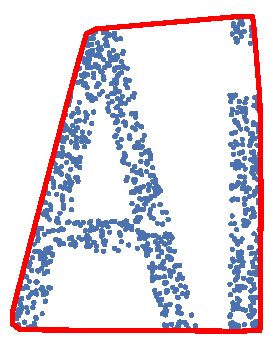
\includegraphics[clip, trim=0.0cm 0.1cm 0.0cm 0.25cm, width=0.20\linewidth]{chapter_2_polylidar/imgs/concave_vs_convex_0.pdf}
    }
    \label{fig:ch1_convex}\hfill
  \subfloat[]{%
  \centering
        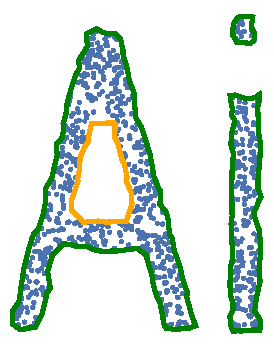
\includegraphics[clip, trim=0.0cm 0.1cm 0.0cm 0.25cm, width=.2\linewidth]{chapter_2_polylidar/imgs/concave_vs_convex_2.pdf}}
    \label{fig:ch1_concave} \hfill
  \subfloat[]{%
    \centering
      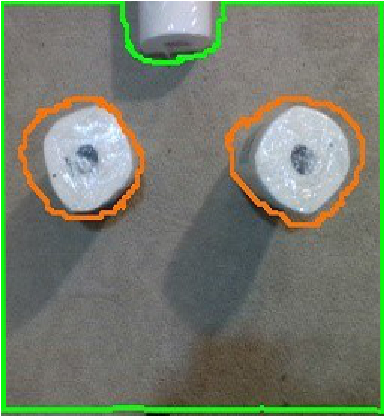
\includegraphics[width=0.25\linewidth]{chapter_2_polylidar/imgs/RealSensePictures-cropped_aspect.pdf}
    }
    \label{fig:ch1_realsense}\hfill\\
  \caption{(a) Convex hull of a point set (red); (b) MultiPolygon extraction using Polylidar (green).
  (c) Polygon extraction from a plane segmented point cloud from an Intel RealSense RGBD camera capturing paper towel rolls on a basement floor. 
  Note that Polylidar also identifies holes (orange).}
  \label{fig:ch1_convex_concave} 
\end{figure}

We show that Polylidar is approximately four times faster than leading open source approaches for concave polygon extraction. Polylidar's speed is attributed to rapidly identifying boundary edges (shell and holes) and then performing  boundary following to ensure a valid polygon is returned. 

\paragraph{Results}
% \section{Experiments}

Polylidar is benchmarked against other common concave hull extraction methods which also extract holes; all code is open source\footnote{https://github.com/JeremyBYU/concavehull-evaluation}. Three other implementations are tested: CGAL's Alpha Shape function and the ST\_ConcaveHull function from PostGIS and Spatialite. For uniformity, Polylidar and CGAL are set to use the same $\alpha$ parameter to guarantee exact shape reproduction. 
Three separate tests sets are created to evaluate the speed and accuracy of each method: plane segmented point clouds produced by an RGBD camera,  synthetic point sets from the state shapes of California (CA) and Hawaii (HI), and synthetic point sets generated form the English alphabet. All tests have a ground truth (multi)polygon, $GT$, to evaluate shape accuracy. Each implementation takes as input a point set and produces a concave shape, $CS$, which is similar to the ground truth polygon.  The $L^2$ error norm, the area of the symmetric difference between $GT$ and $CS$, is computed to enable evaluation of shape error $\frac{area((GT-CS) \cup (CS-GT))}{area(CS)}$. For brevity only the results of the alphabet shapes are shown in this summary. 



% \subsection{Alphabet Shapes}\label{sec:alphabet_shapes}

% {\color{blue}
Polygons from 26 capital letters of the English alphabet were generated and 2000 points randomly sampled inside.
%Some polygon letters naturally have holes such as ``A'', however no capital letters are MultiPolygons. Each letter was uniformly sampled to generate a 2000 point set and run through each algorithm. 
The ``A'' in Figure \ref{fig:ch1_convex_concave}b shows an example capital letter with the output of Polylidar's concave hull. Table \ref{table:alphabet_tests} provides aggregate statistics of all 26 test cases. Polylidar is about four times faster than the second fastest algorithm CGAL. Spatialite has marginally higher accuracy then both CGAL and Polylidar. 
% The alphabet shapes are significantly more concave than previous benchmarks. Documentation of PostGIS indicates that the run time grows quadratically as concavity increases leading to the high execution times observed \cite{open_source_geospatial_foundation_postgis_2019}.

%However PostGIS shape error and time are significantly higher than previously seen. This is because the alphabet shapes are significantly more concave then the tested state shapes, requiring a much smaller \emph{target percent} parameter for PostGIS (on average 0.38). Documentation of PostGIS indicates that the run time grows quadratically when reducing this parameter and at ``small'' values may fail to produce a concave shape \cite{postgis}.  PostGIS failed to produce any shape for the letters ``J'', ``L'', and ``M''. All other algorithms provided valid results for all test cases.
%  (reduced to 1000 points for visual clarity)

%  Polylidar continues to lead in speed, about 4.5 times faster than the next leading algorithm CGAL (shape error remains the same because of same $\alpha$ used). Spatialite continues to lead in accuracy by a marginal amount for the same reasons discussed previously. However PostGIS shape error and time are significantly higher than previously seen. This is because the alphabet shapes are significantly more concave then the tested state shapes, requiring a much smaller \emph{target percent} parameter for PostGIS (on average 0.38). 
% Documentation of PostGIS indicates that the run time grows quadratically when reducing this parameter and at ``small'' values may fail to produce a concave shape \cite{postgis}.  PostGIS failed to produce any shape for the letters ``J'', ``L'', and ``M''. All other algorithms provided valid results for all test cases.
% }
 
\begin{table}[!ht]
\centering
\caption{Alphabet Letter Results, 26 Shapes}
\label{table:alphabet_tests}
\begin{tabular}{lcccccc}
\toprule
{} & \multicolumn{3}{c}{$L^2$ error \%} & \multicolumn{3}{c}{Time (ms)} \\
{Algorithm} &    mean & std &  max &      mean &     std &     max \\
% Algorithm        &         &     &      &           &         &         \\
\midrule
% polylidar  &    12.8 & 1.8 & 16.8 &       1.8 &     0.3 &     2.9 \\
% cgal       &    12.8 & 1.8 & 16.8 &       6.8 &     0.8 &     9.8 \\
% postgis    &    36.5 & 9.9 & 53.7 &   18973.3 & 10786.2 & 39587.8 \\
% spatialite &    11.2 & 4.5 & 22.1 &     330.4 &    33.8 &   438.1 \\
Polylidar  &           12.8 & \textbf{1.8} & \textbf{16.8} &       \textbf{1.2} &    \textbf{0.3} &     \textbf{2.4} \\
CGAL       &           12.8 & \textbf{1.8} & \textbf{16.8} &       5.4 &    0.9 &     7.2 \\
PostGIS    &           36.5 & 9.9 & 53.7 &   13091.8 & 7500.6 & 28451.0 \\
Spatialite &           \textbf{11.2} & 4.5 & 22.1 &     230.2 &    6.3 &   242.9 \\
\bottomrule
\end{tabular}
\end{table}


\paragraph{Conclusion}
This chapter introduces Polylidar, an efficient 2D concave hull extraction algorithm that produces (multi)polygon output with holes. Comparison benchmarks of numerous test sets, similarly done in \cite{duckham_efficient_2008}, show Polylidar is faster than competing approaches with comparable or better accuracy. A full description of the algorithm with additional results is available in \cite{castagno_polylidar_2020}.


% Contributions of this chapter are:
% \begin{itemize}
%   \item A faster open source \cite{Castagno_Github_Polylidar} concave (multi)polygon extraction algorithm from 2D point sets.
%   \item A benchmark comparison of leading concave polygon extraction techniques in terms of accuracy and speed.
% \end{itemize}


% Below, Sections \ref{sec:background} and \ref{sec:prelim} provide background on non-convex shape generation and mathematical preliminaries, respectively. Section \ref{sec:methods} describes Polylidar algorithms, while Section \ref{sec:results} shows benchmark test results of Polylidar versus other methods.  Section \ref{sec:random_polygons_test} describes test results. Sections  \ref{sec:discussion} and \ref{sec:conclusion} provide discussion and conclusions.



% \section{Background}\label{sec:background}

% Characterizing the shape of a set of 2D points $\mathcal{P}$ has been a long-term focus of computational geometry research. A convex hull is defined as the smallest convex polygon that fully encapsulates all points in a set $\mathcal{P}$.  Although widely used to estimate shape, point sets with non-convex distributions are poorly characterized by a convex hull \cite{duckham_efficient_2008}.  Convex hull over-estimation can be a serious issue when the points represent physical objects, e.g., obstacle free navigable areas. Several algorithms have been developed to construct shapes that ``fit'' or ``cover'' point sets more closely. 

% Figure \ref{fig:ch1_convex_concave} compares convex and concave hulls. Figure \ref{fig:ch1_convex_concave}b is the multipolygon output of Polylidar described below.
% %One may argue that the red convex hull does not conform well to the point distribution but the green concave hull captures the shape of the letters more precisely. 
% While there is a unique convex hull, there is no true or unique concave hull.  Concave hull algorithm implementations can also have different output types.  Some return only an unordered set of edges while others return a single polygon.  Some algorithms return multiple disconnected polygons (multipolygon), and some can generate holes inside a polygon.

% The $\alpha$-shape algorithm is an early strategy to generate a family of shapes ranging from a convex hull to a point set  \cite{edelsbrunner_shape_1983}. The parameter $\alpha$ dictates the radius of a closed disk used to prune/remove area in the convex hull. This disk is allowed to move freely shaving off the excess shape until it finds points. When disk radius is large, ideally infinite, the convex hull is produced; when disk radius is infinitesimally small only the points remain. A common implementation of $\alpha$-shape organizes points using Delaunay triangulation and filters triangles whose circumcircle radius is less than $\alpha$.  The final shape is represented by the remaining edges and triangles.  Note that the $\alpha$-shape method creates multiple non-intersecting shapes with the possibility of holes. 

% % The algorithm in \cite{Duckham2008} produces polygons from point sets called $\chi$-shapes. Like some $\alpha$-shape implementations, the $\chi$-shape approach begins with Delaunay triangulation to order and spatially connect data points.  The algorithm differs by iteratively removing the longest exterior edges from triangulation based on a specified maximum length parameter $l$. A corner case occurs  when edge removal results in a non-simple polygon, i.e., the polygon wraps into itself; in this case edge removal is skipped.  The $\chi$-shape produced is a single polygon with no possibility of holes.

% The geospatial software library Spatialite \cite{furieri_spatialite_2017}, an extension to SQLite \cite{hipp_sqlite_2020}, contains a concave hull extraction procedure. The algorithm again starts with Delaunay triangulation then analyzes the distribution of each triangle's edge length to determine mean $\mu_l$ and standard deviation $\sigma_l$. Any triangle with edge length greater than $C \cdot \sigma_l  + \mu_l$ is removed, where $C$ is a user-defined parameter. The final geometry returned is the union of all triangles computed with GEOS, a high performance open source geometry engine. The output may be a multipolygon (i.e., multiple disjoint polygons) with the possibility of holes inside each. 

% PostGIS is a geospatial database of computational geometry routines such as the concave hull method in \cite{open_source_geospatial_foundation_postgis_2019}. This algorithm first calculates the convex hull and then shrinks the hull by adjusting vertex connections to closer points which ``cave in'' the hull.  This process recursively shrinks a boundary until a user-specified percent reduction in area from the convex hull is achieved. The resulting shape is a single polygon with the possibility of holes. 

% \begin{table}[ht]
% \centering
% \caption{Concave Hull Extraction Methods}
% \label{table:compare_alg}
% \begin{tabular}{ccc}
% \hline
% Algorithm                                                   & Output                                                           & Holes? \\ \hline
% \begin{tabular}[c]{@{}c@{}}CGAL $\alpha$-shape\end{tabular}   & \begin{tabular}[c]{@{}c@{}}unordered\\ set of edges\end{tabular} & Yes    \\
% % $\chi$-shapes                                             & \begin{tabular}[c]{@{}c@{}}Unordered\\ Set of Edges\end{tabular} & No     \\
% Spatialite                                                 & (multi)polygon                                                   & Yes    \\
% PostGIS                                                       & polygon                                                          & Yes    \\
% Polylidar (new)                                                   & (multi)polygon                                                   & Yes    \\ \hline
% \end{tabular}
% \end{table}

% Table \ref{table:compare_alg} provides a summary  of the concave hull algorithms discussed above. The Computational Geometry Algorithms Library (CGAL) is  used as the implementation of the $\alpha$-shape method \cite{the_cgal_project_cgal_2019}. Note that the time complexity of all algorithm implementations, with the exception of PostGIS, is $\mathcal{O}(n\log{}n)$.  Our paper contributes a procedure to more rapidly compute (multi)polygon output with the possibility of holes.  Though this is a complex output to generate, we show through benchmarks that our algorithm and implementation outperforms other available approaches.

% \section{Preliminaries}\label{sec:prelim}

% A 2D \textit{point set} is an arbitrarily ordered set of two dimensional points in a Cartesian reference frame. Each point is defined by orthogonal bases $\hat{\mathbf{e}}_x$ and $\hat{\mathbf{e}}_y$  with
% \begin{equation}
% \label{eq:point}
%     \vec{{p}_{i}}=x\,\hat{\mathbf{e}}_x+y\, \hat{\mathbf{e}}_y= [x,y]
% \end{equation}
% where $x,y$ are plane coordinates.

% An $n$-point array $\mathcal{P} = \{ \vec{{p}_{1}}, \vec{{p}_{i}}, \ldots, \vec{{p}_{n}} \}$ contains points $\vec{{p}_{i}} \in \mathbb{R}^2$ indexed by $i$.  A triangular mesh $ \mathcal{T}$ is defined by
% \begin{equation}
% \label{eq:tri}
%     \mathcal{T} = \{ t_1, t_i, \ldots, t_{k} \}
% \end{equation}
% where each $t_i$ is a triangle with vertices defined by three point indices $\{i_1, i_2, i_3\} \in \left[1,n\right]$ referencing points in $\mathcal{P}$.

% We follow the Open Geospatial Consortium (OGC) standard \cite{herring_opengis_2006-1} for defining \textit{linear ring} and \textit{polygon}. A linear ring is a consecutive list of points that is both closed and simple. This requires a linear ring to have non-intersecting line segments that join to form a closed path. The key components of a valid polygon are a single exterior linear ring representing the \emph{shell} of the polygon and a set of linear rings (possibly empty) representing \emph{holes} inside the polygon. 